\section{Produkteinsatz}

In diesem Abschnitt wird der geplante Einsatz des Systems beschrieben, wobei insbesondere auf die Systemumgebung, in der das Produkt eingesetzt werden soll, und die Zuordnung der Software zu dieser eingegangen wird. Abbildung \ref{ProdukteinsatzKomp} zeigt ein Verteilungsdiagramm des Gesamtsystems, dessen Komponenten im Folgenden erläutert werden.

Das Gesamtsystem besteht aus einem \emph{Server}, der mit mindestens einem \emph{Robot} verbunden ist, wobei zwischen \emph{Server} und \emph{Robot} über einen auf beiden Seiten entsprechend verfügbaren \emph{IWlan\-Adapter} über ein Funknetzwerk kommuniziert werden kann. \emph{Robots} können nicht mit anderen \emph{Robots} kommunizieren.

Auf dem \emph{Server} und den \emph{Robots} läuft ein \emph{Java Runtime Environment}, das dem Ausführen der entsprechenden Software dient.

\emph{Robot.jar} dient der Kapselung der verfügbaren Funktionen. Es werden auch die \emph{Interfaces} zusammengefasst, die dem Ansprechen von \emph{INorthStar}, \emph{IDrive}, \emph{IBumper}, \emph{IBumperHandler}, \emph{IDistanceSensor} und \emph{IBattery} dienen.

\emph{Server.jar} funktioniert analog zu \emph{Robot.jar} und stellt alle grundlegenden Funktionen zur Verfügung. Dazu gehören insbesondere auch die Komponenten \emph{Hospital}, und \emph{NetworkAccess}.

Zusätzlich benötigte Funktionalitäten werden aus dem Common-Paket importiert und sind sowohl bei \emph{Robots} als auch dem \emph{Server} verfügbar.

\begin{figure}[H]
	\centering
	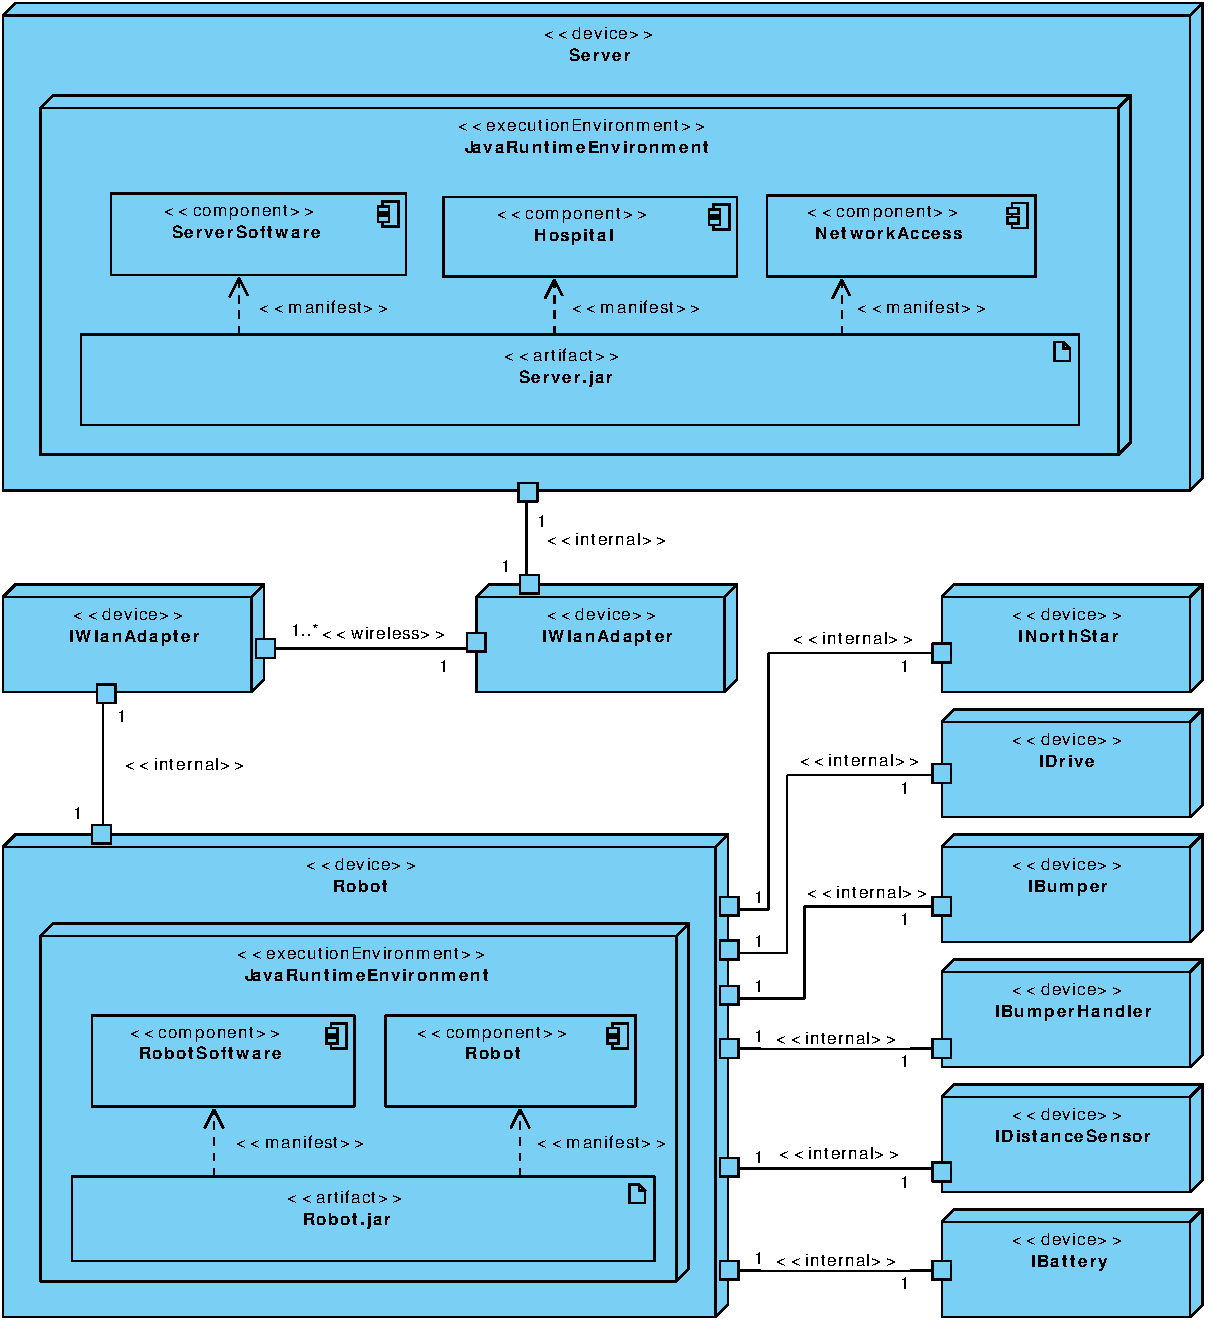
\includegraphics[width=1\textwidth]{img/1-Entwurf-9-Produkteinsatz}
	\caption{Verteilungsdiagramm des Gesamtsystems}
	\label{ProdukteinsatzKomp}
\end{figure}